% Figure: CNS Energy Triage Hierarchy
% Shows priority levels for CNS functions under energy scarcity

\begin{figure}[htbp]
\centering
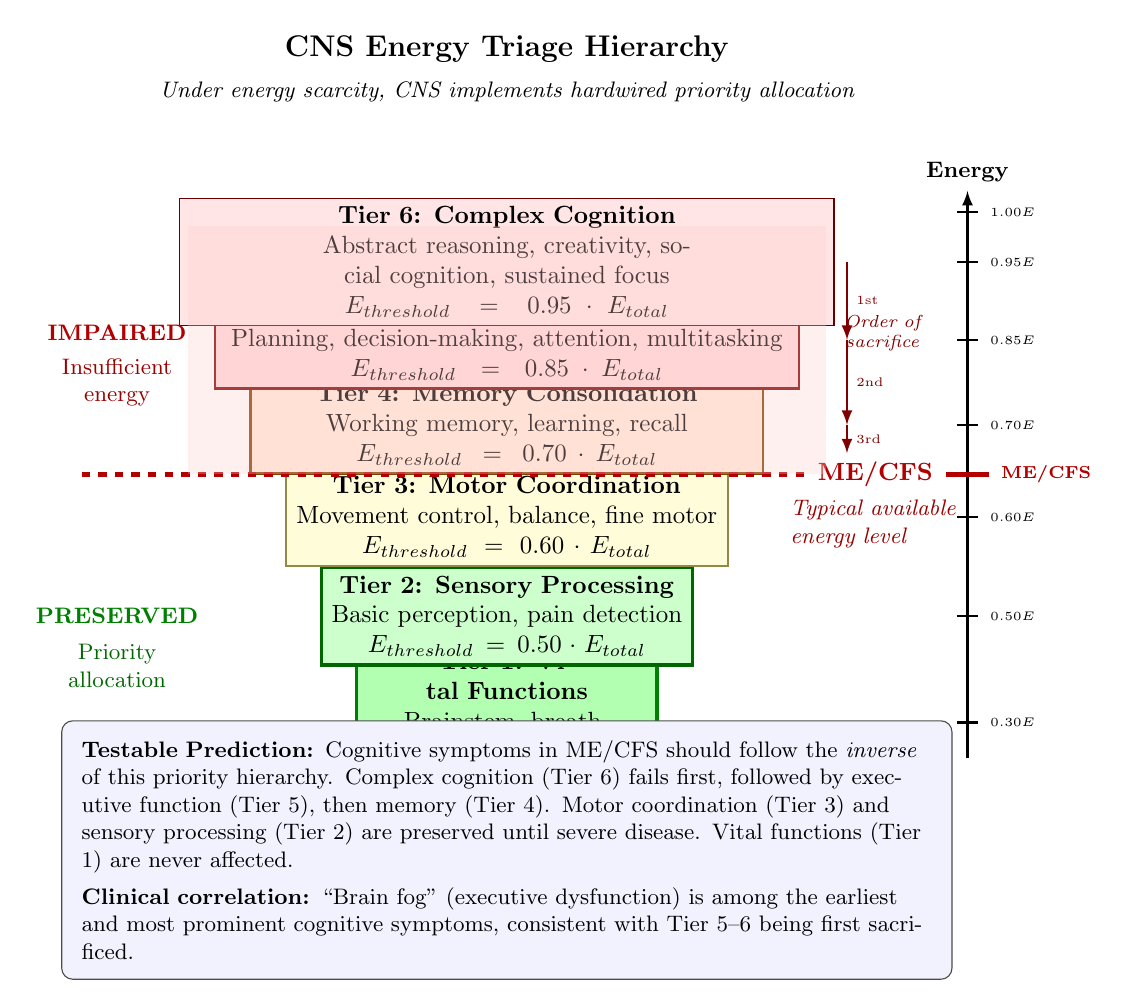
\begin{tikzpicture}[
    scale=0.9, every node/.style={scale=0.9},
    % Tier styles (darker = higher priority)
    tier1/.style={draw=green!50!black, fill=green!30, very thick, text width=4cm, align=center, minimum height=1.2cm},
    tier2/.style={draw=green!40!black, fill=green!20, very thick, text width=5cm, align=center, minimum height=1.1cm},
    tier3/.style={draw=yellow!50!black, fill=yellow!15, thick, text width=6cm, align=center, minimum height=1cm},
    tier4/.style={draw=orange!50!black, fill=orange!15, thick, text width=7cm, align=center, minimum height=1cm},
    tier5/.style={draw=red!50!black, fill=red!15, thick, text width=8cm, align=center, minimum height=1cm},
    tier6/.style={draw=red!40!black, fill=red!10, text width=9cm, align=center, minimum height=0.9cm},
    % Energy line
    energy-line/.style={ultra thick, dashed, red!70!black},
    % Threshold labels
    threshold/.style={font=\scriptsize\bfseries, fill=white, inner sep=2pt},
]

% Title
\node[font=\large\bfseries] at (0, 9.5) {CNS Energy Triage Hierarchy};
\node[font=\small\itshape] at (0, 8.9) {Under energy scarcity, CNS implements hardwired priority allocation};

% === PYRAMID TIERS (bottom to top = highest to lowest priority) ===

% Tier 1: Vital (never sacrificed)
\node[tier1] (t1) at (0, 0) {\textbf{Tier 1: Vital Functions}\\Brainstem, breathing, cardiac rhythm\\$E_{min} = 0.30 \cdot E_{total}$};

% Tier 2: Critical
\node[tier2] (t2) at (0, 1.5) {\textbf{Tier 2: Sensory Processing}\\Basic perception, pain detection\\$E_{threshold} = 0.50 \cdot E_{total}$};

% Tier 3: Important
\node[tier3] (t3) at (0, 2.9) {\textbf{Tier 3: Motor Coordination}\\Movement control, balance, fine motor\\$E_{threshold} = 0.60 \cdot E_{total}$};

% Tier 4: Standard
\node[tier4] (t4) at (0, 4.2) {\textbf{Tier 4: Memory Consolidation}\\Working memory, learning, recall\\$E_{threshold} = 0.70 \cdot E_{total}$};

% Tier 5: Non-essential
\node[tier5] (t5) at (0, 5.4) {\textbf{Tier 5: Executive Function}\\Planning, decision-making, attention, multitasking\\$E_{threshold} = 0.85 \cdot E_{total}$};

% Tier 6: Luxury
\node[tier6] (t6) at (0, 6.5) {\textbf{Tier 6: Complex Cognition}\\Abstract reasoning, creativity, social cognition, sustained focus\\$E_{threshold} = 0.95 \cdot E_{total}$};

% === ME/CFS ENERGY LINE ===
\draw[energy-line] (-6, 3.5) -- (6, 3.5);
\node[font=\bfseries, red!70!black, fill=white, inner sep=3pt] at (5.2, 3.5) {ME/CFS};
\node[font=\small\itshape, red!60!black, text width=3cm, align=left] at (5.5, 2.8) {Typical available\\energy level};

% === SHADING FOR AFFECTED TIERS ===
\fill[red!20, opacity=0.3] (-4.5, 3.5) rectangle (4.5, 7);

% Labels for affected vs preserved
\node[font=\small\bfseries, red!70!black] at (-5.5, 5.5) {IMPAIRED};
\node[font=\small, red!60!black, text width=2cm, align=center] at (-5.5, 4.8) {Insufficient energy};

\node[font=\small\bfseries, green!50!black] at (-5.5, 1.5) {PRESERVED};
\node[font=\small, green!40!black, text width=2cm, align=center] at (-5.5, 0.8) {Priority allocation};

% === ENERGY SCALE (right side) ===
\begin{scope}[xshift=6.5cm]
    \draw[thick, -latex] (0, -0.5) -- (0, 7.5) node[above, font=\small\bfseries] {Energy};

    % Markers
    \foreach \y/\val in {0/0.30, 1.5/0.50, 2.9/0.60, 4.2/0.70, 5.4/0.85, 6.5/0.95, 7.2/1.00} {
        \draw[thick] (-0.15, \y) -- (0.15, \y);
        \node[right, font=\tiny] at (0.2, \y) {$\val E$};
    }

    % ME/CFS marker
    \draw[red!70!black, ultra thick] (-0.3, 3.5) -- (0.3, 3.5);
    \node[right, font=\scriptsize\bfseries, red!70!black] at (0.35, 3.5) {ME/CFS};
\end{scope}

% === PREDICTION BOX ===
\node[draw=black!70, fill=blue!5, rounded corners, text width=12cm, align=left, font=\small, inner sep=8pt] at (0, -1.8) {
\textbf{Testable Prediction:} Cognitive symptoms in ME/CFS should follow the \emph{inverse} of this priority hierarchy. Complex cognition (Tier 6) fails first, followed by executive function (Tier 5), then memory (Tier 4). Motor coordination (Tier 3) and sensory processing (Tier 2) are preserved until severe disease. Vital functions (Tier 1) are never affected.\\[4pt]
\textbf{Clinical correlation:} ``Brain fog'' (executive dysfunction) is among the earliest and most prominent cognitive symptoms, consistent with Tier 5--6 being first sacrificed.
};

% === ARROWS showing sacrifice order ===
\draw[-latex, thick, red!50!black] (4.8, 6.5) -- (4.8, 5.4) node[midway, right, font=\tiny] {1st};
\draw[-latex, thick, red!50!black] (4.8, 5.4) -- (4.8, 4.2) node[midway, right, font=\tiny] {2nd};
\draw[-latex, thick, red!50!black] (4.8, 4.2) -- (4.8, 3.8) node[midway, right, font=\tiny] {3rd};

\node[font=\scriptsize\itshape, red!50!black, text width=1.5cm, align=center] at (5.3, 5.5) {Order of sacrifice};

\end{tikzpicture}
\caption{CNS energy triage hierarchy under energy scarcity. The red dashed line indicates typical available energy in ME/CFS. Functions above the line (Tiers 4--6) are impaired; functions below (Tiers 1--3) are preferentially preserved through energy allocation.}
\label{fig:energy-triage-hierarchy}
\end{figure}
